\chapter{Ανάλογα ποσά - Αντιστρόφως ανάλογα ποσά}
\begin{exercise}
Να σχεδιάσεις ένα ορθοκανονικό σύστημα ημιαξόνων, με μονάδα το 1 cm και να
τοποθετήσεις τα σημεία Α(2,3), Β(3,2), Γ(4,5), Δ(5,5), Ε(1,4), Z(7,3), Η(7,2), Θ(6,2),
Ι(6,0), Κ(0,5). Τι παρατηρείς για τα σημεία Ι και Κ; Πού βρίσκονται αυτά; Μπορείς να
γενικεύσεις τις παρατηρήσεις σου για τα σημεία που έχουν τετμημένη ή τεταγμένη το
μηδέν;
\end{exercise}
\begin{lstlisting}
import matplotlib.pyplot as plt

plt.clf()
points = [(2,3), (3,2), (4,5), (5,5), (1,4), (7,3), (7,2), (6,2), (6,0), (0,5)]
pointName = ['Α','Β','Γ','Δ','Δ','Ε','Ζ','Η','Θ','Ι','Κ']
x = [p[0] for p in points]
y = [p[1] for p in points]
color=['m','g','r','b']
plt.grid()
plt.scatter(x,y, s=100 ,marker='o', c=color)
for (i,p) in enumerate(points):
    plt.annotate(pointName[i],(p[0],p[1]))

plt.show()
\end{lstlisting}
\begin{figure}
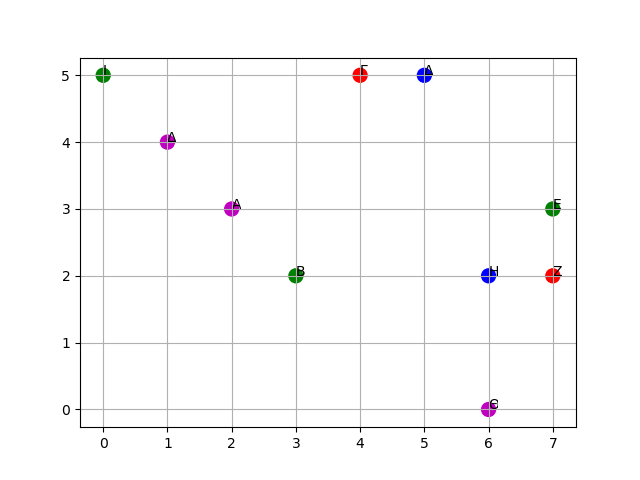
\includegraphics{graph1.png}
\end{figure}
